%!TEX program = xelatex
\documentclass[10pt, compress]{beamer}
\usetheme[titleprogressbar]{m}

\usepackage{booktabs}
\usepackage[scale=2]{ccicons}
\usepackage{minted}
\usepackage{graphicx}
\graphicspath{ {images/} }

\usepgfplotslibrary{dateplot}

\usemintedstyle{trac}

\title{proper motions}
\subtitle{How Do The Faintest Of Stars Move}
\date{July 29,2015}
\author{Prashansa Gupta}
\institute{Indian Institute of Science Education and Research, Mohali, India}

\begin{document}

\maketitle

%%%%%%%%%%%%%%%%%%%%%%%%%%%%%%%%%%%%%%
\section{Problem Statement}

\begin{frame}[fragile]
  \frametitle{Objective}
  We wish to look at the faintest of stars in the sky and investigate their kinematics. 
\end{frame}  


%%%%%%%%%%%%%%%%%%%%%%%%%%%%%%%%%%%%%%
\section{Motivation}

\begin{frame}
\frametitle{Two Ways}
	There are two ways in which one can approach the problem. 
	\begin{enumerate}
		\item<1-> Take high precision data over a short period of time
        \item<2-> Or wait long enough so that a compromise over precision can be made
	\end{enumerate}

\end{frame}

\begin{frame}
\frametitle{First way}
	\begin{itemize}
    	\item<1-> \textsc{Hipparcos}(HIgh Precision PARallax COllecting Satellite) 
        		\begin{itemize}
                	\item<2-> high precision data taken over $3$ years
                    \item<3-> a $100,000$ stars were observed upto $12.4$ magnitude 					\item<4-> proper motion accuracy of $0.88 mas/yr$ in RA and $0.74 mas/yr$ in DEC with systematic errors $< 0.1mas$.
                \end{itemize}   
    	\item<5-> The GAIA mission 
        		\begin{itemize}
                	\item<6-> even fainter stars - complete upto $20$th magnitude
                    \item<7->a billion stars with an accuracy of about $20 \mu as$ at $15$ mag, and $200 \mu as$ at $20$ mag.
                 \end{itemize}   
    \end{itemize}
\end{frame}

\begin{frame}
\frametitle{First way}
But their still remains one shortcoming, they do not give data for fainter stars beyond $20$th magnitude. 

There are quite a lot of stars even between $20$ and $21$ magnitude. Roughly estimated, for RR lyrae stars, these magnitudes translate to 92 and 120 kpc. One can easily see how big a volume of the sky are we missing out on! 

\end{frame}


\begin{frame}
\frametitle{second way}
	\begin{itemize}
    	\item<1-> we use data that spans 60 years (PanStarrs+SDSS+POSS)
        \item<2-> different catalogs have different astrometric calibration - we need to calibrate them to the same reference system defined by PS1 galaxies. 

        %A rough estimate of the expected uncertainty will be $\sim 20 mas$ which goes down to $\sim 2 mas$ with the averaging over a hundred galaxies. 
    \end{itemize}
\end{frame}


% Positions provided by different catalogs over such a long time frame enable us to determine proper motion with a negligible compromise on uncertainties.

%%%%%%%%%%%%%%%%%%%%%%%%%%%%%%%%%%%%%%
\section{Method Proposed}

\begin{frame}
\frametitle{Method Proposed}
	\begin{enumerate}
		\item<1-> begin with  the PanStarrs dataset
        \item<2-> Obtain a fixed background of galaxies : The Reference System
        	\begin{itemize}
				\item<3-> The data does seem to suggest that the galaxies 'move'
                \item<4-> four epochs, \begin{figure}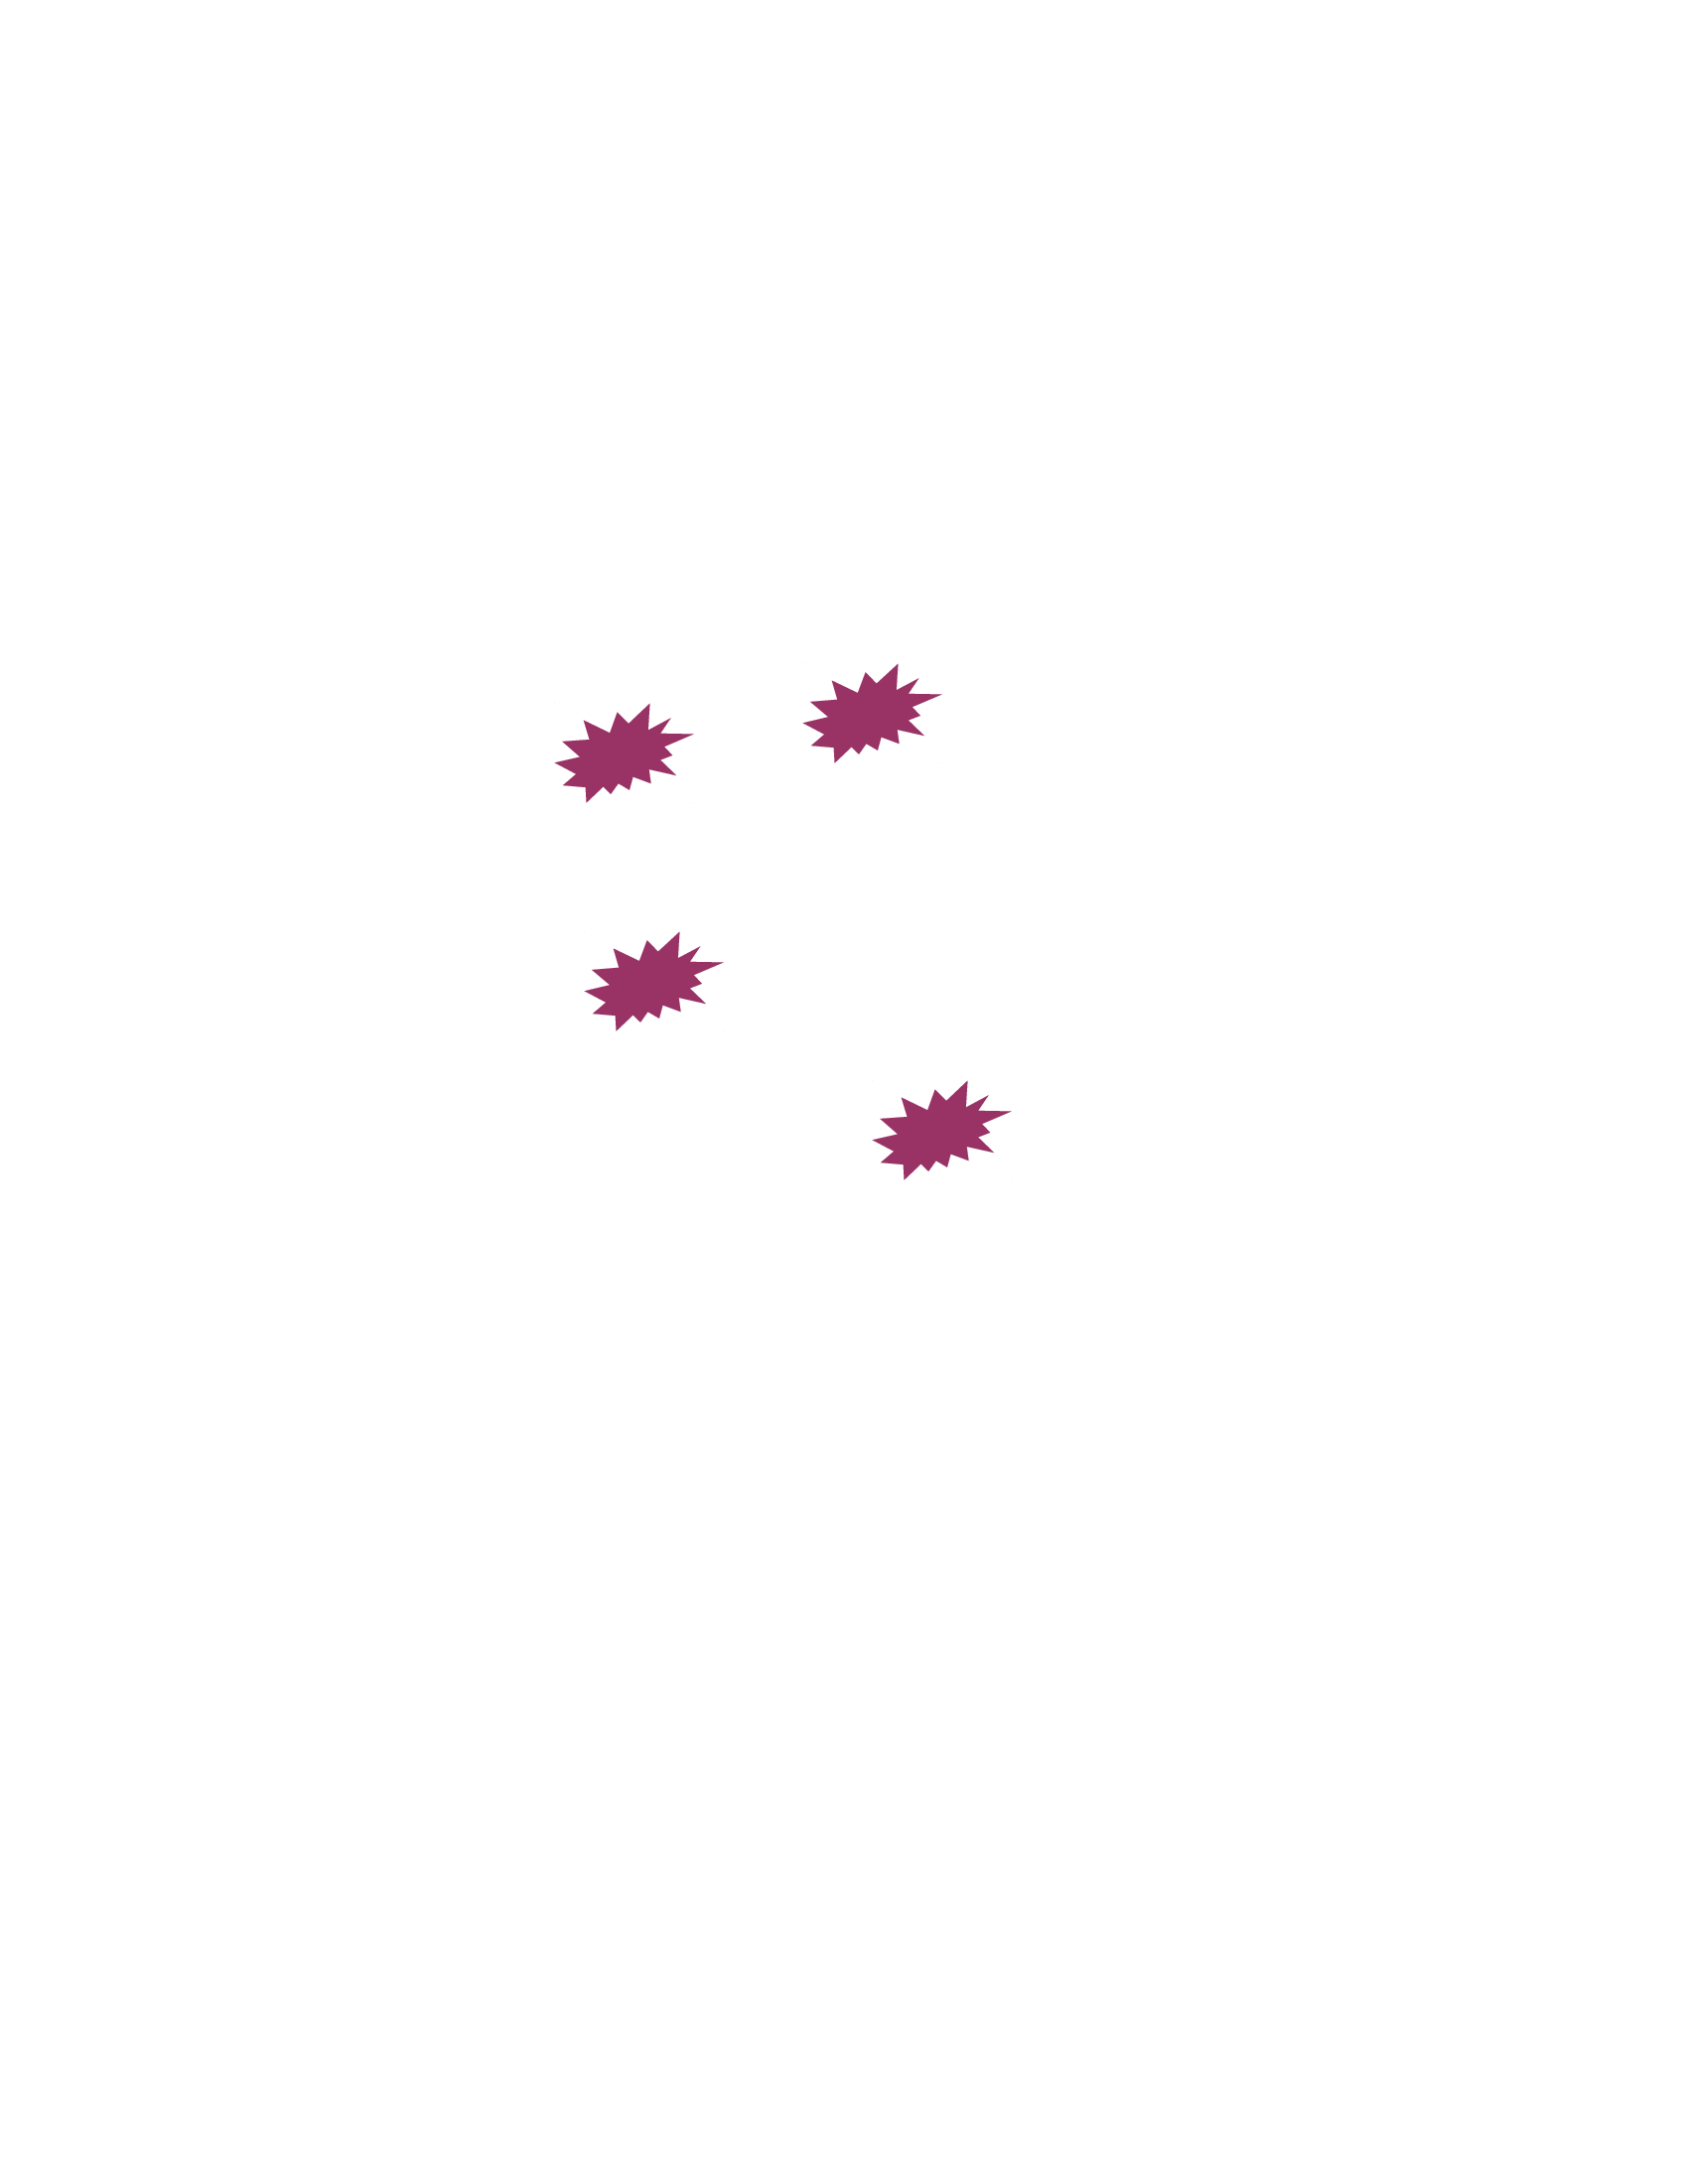
\includegraphics[width=0.5\textwidth]{1.jpg}
                \end{figure}          
            \end{itemize}
      \end{enumerate}      
				
\end{frame}             
                
\begin{frame}
\frametitle{Method Proposed}
	\begin{enumerate}
		\item begin with  the PanStarrs dataset
        \item Obtain a fixed background of galaxies : The Reference System
        	\begin{itemize}
				\item The data does seem to suggest that the galaxies 'move'
            	\item four epochs, find a median value, \begin{figure}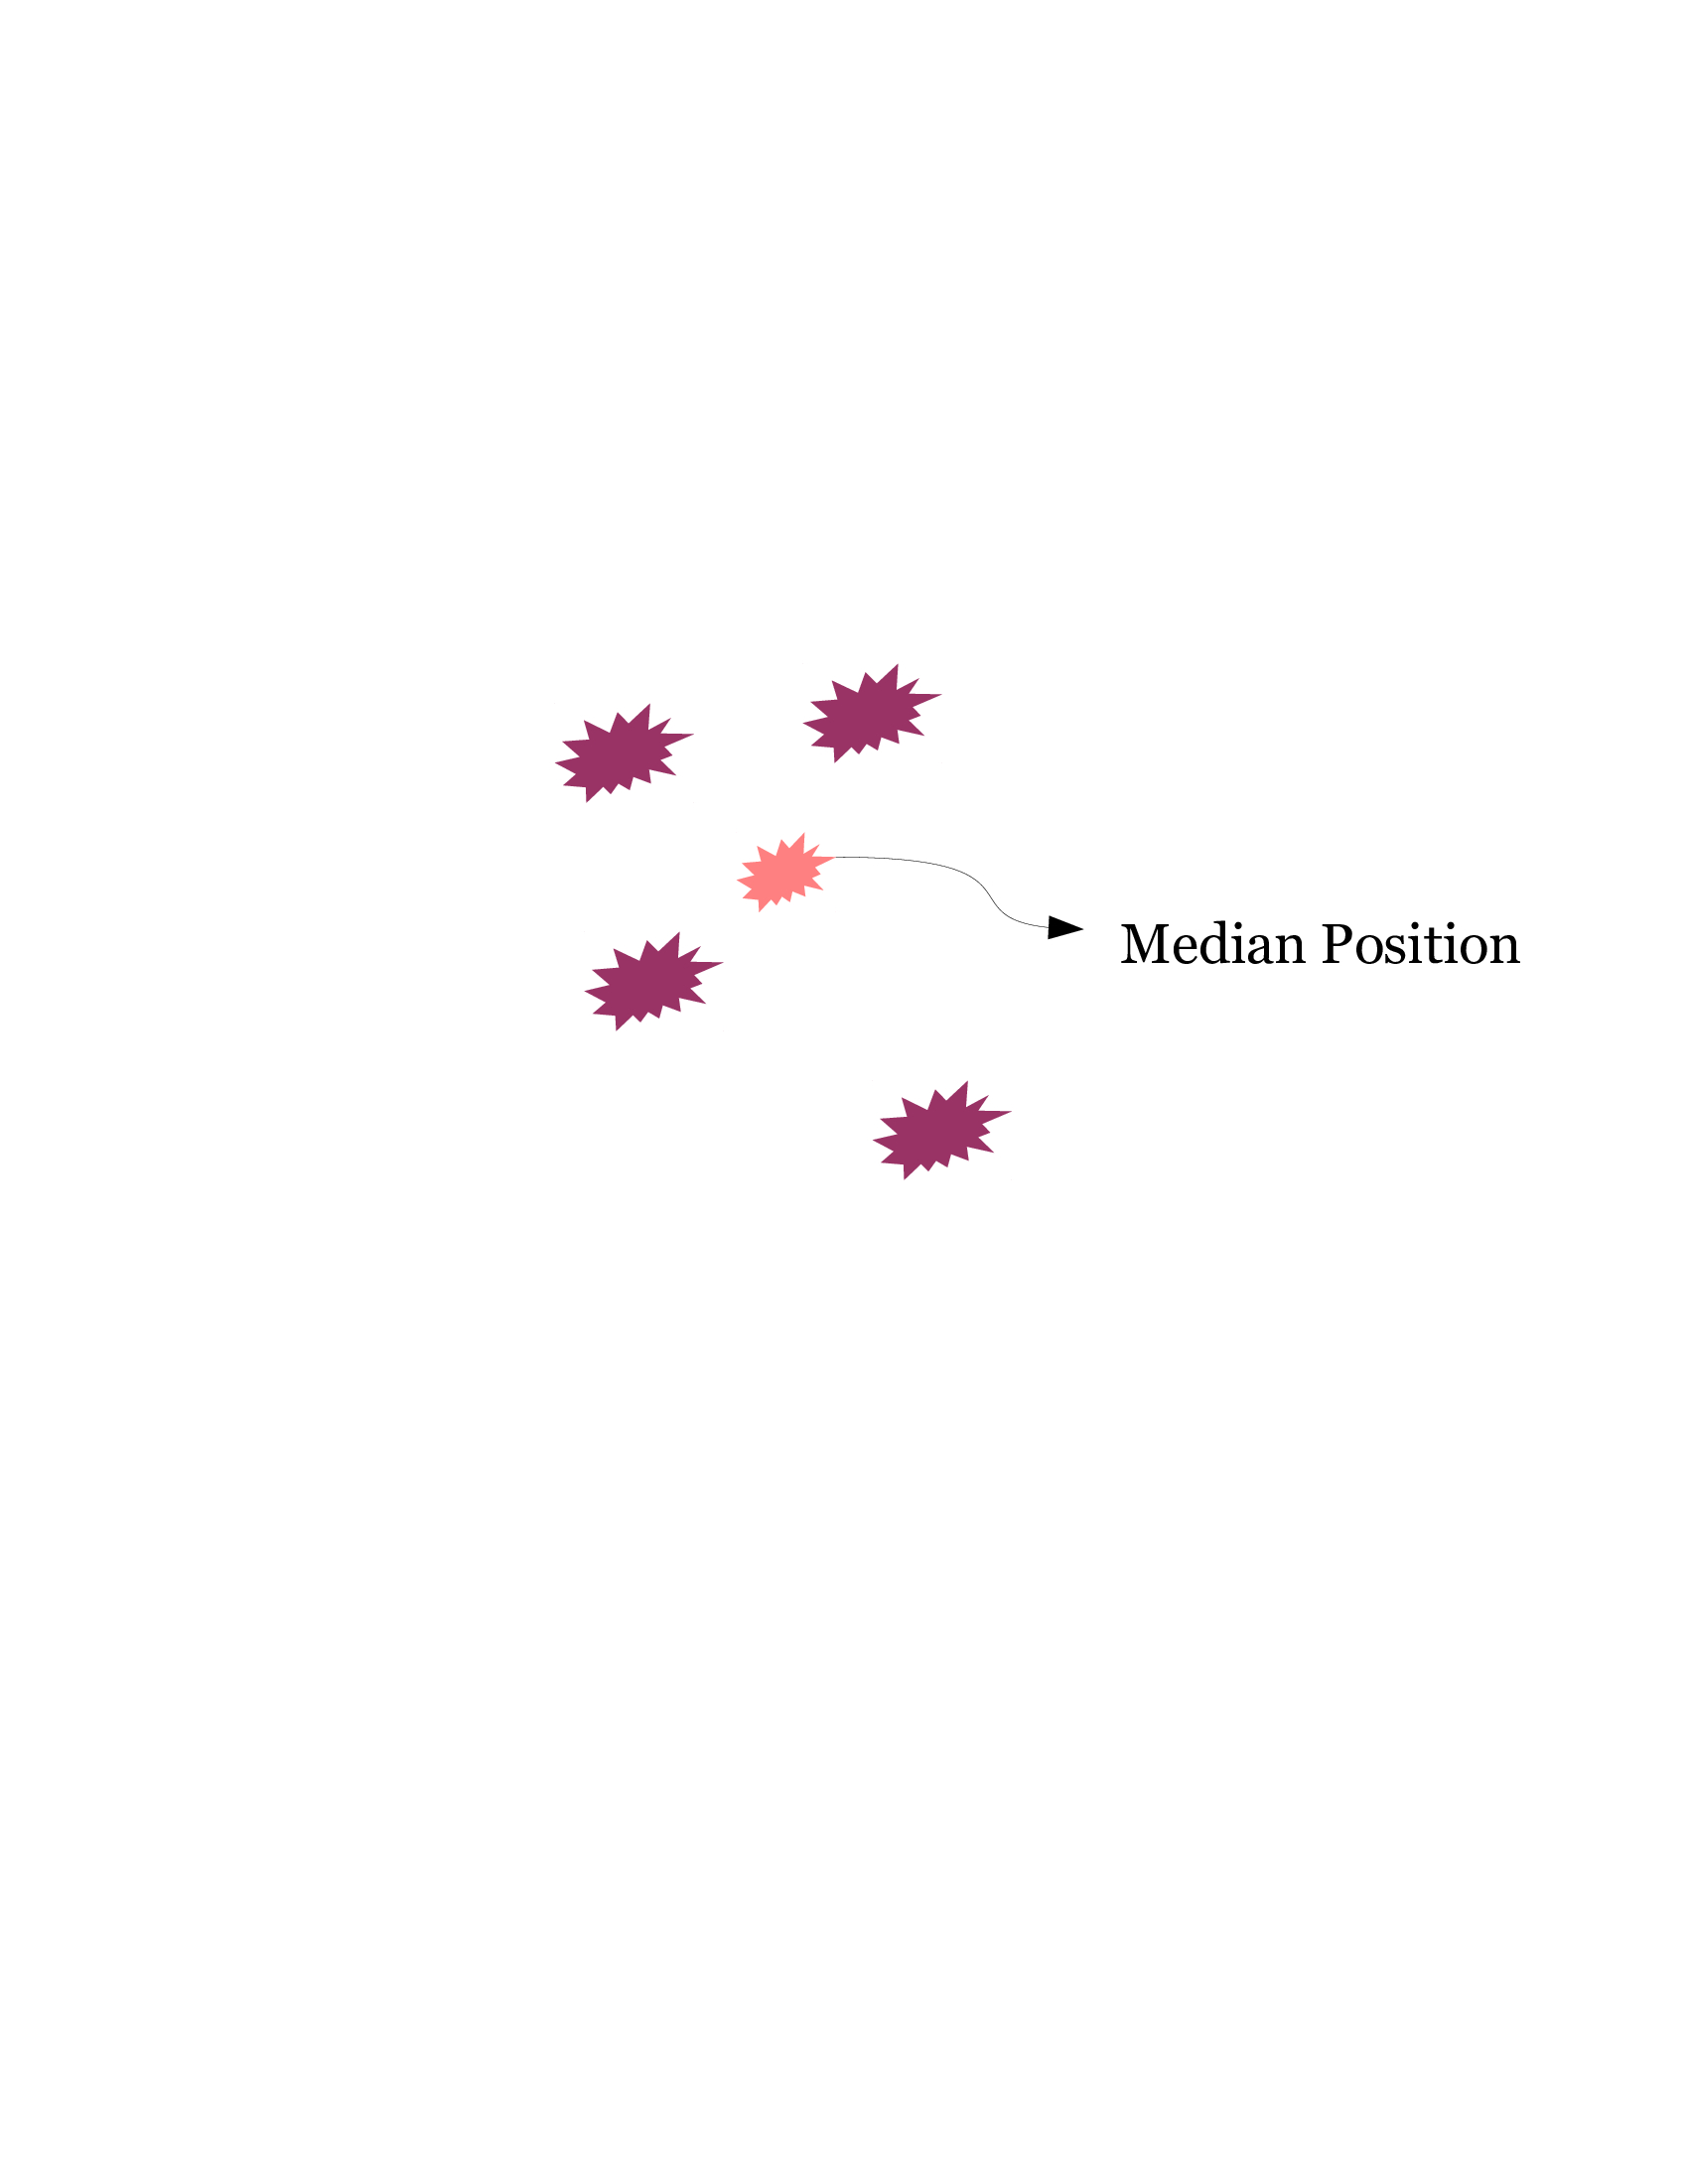
\includegraphics[width=0.5\textwidth]{2.jpg} \end{figure}
             \end{itemize}
      \end{enumerate}
      
\end{frame}

               
\begin{frame}
\frametitle{Method Proposed}
	\begin{enumerate}
		\item begin with  the PanStarrs dataset
        \item Obtain a fixed background of galaxies : The Reference System
        	\begin{itemize}
				\item The data does seem to suggest that the galaxies 'move'
				\item four epochs, find a median value, find offsets, \begin{figure}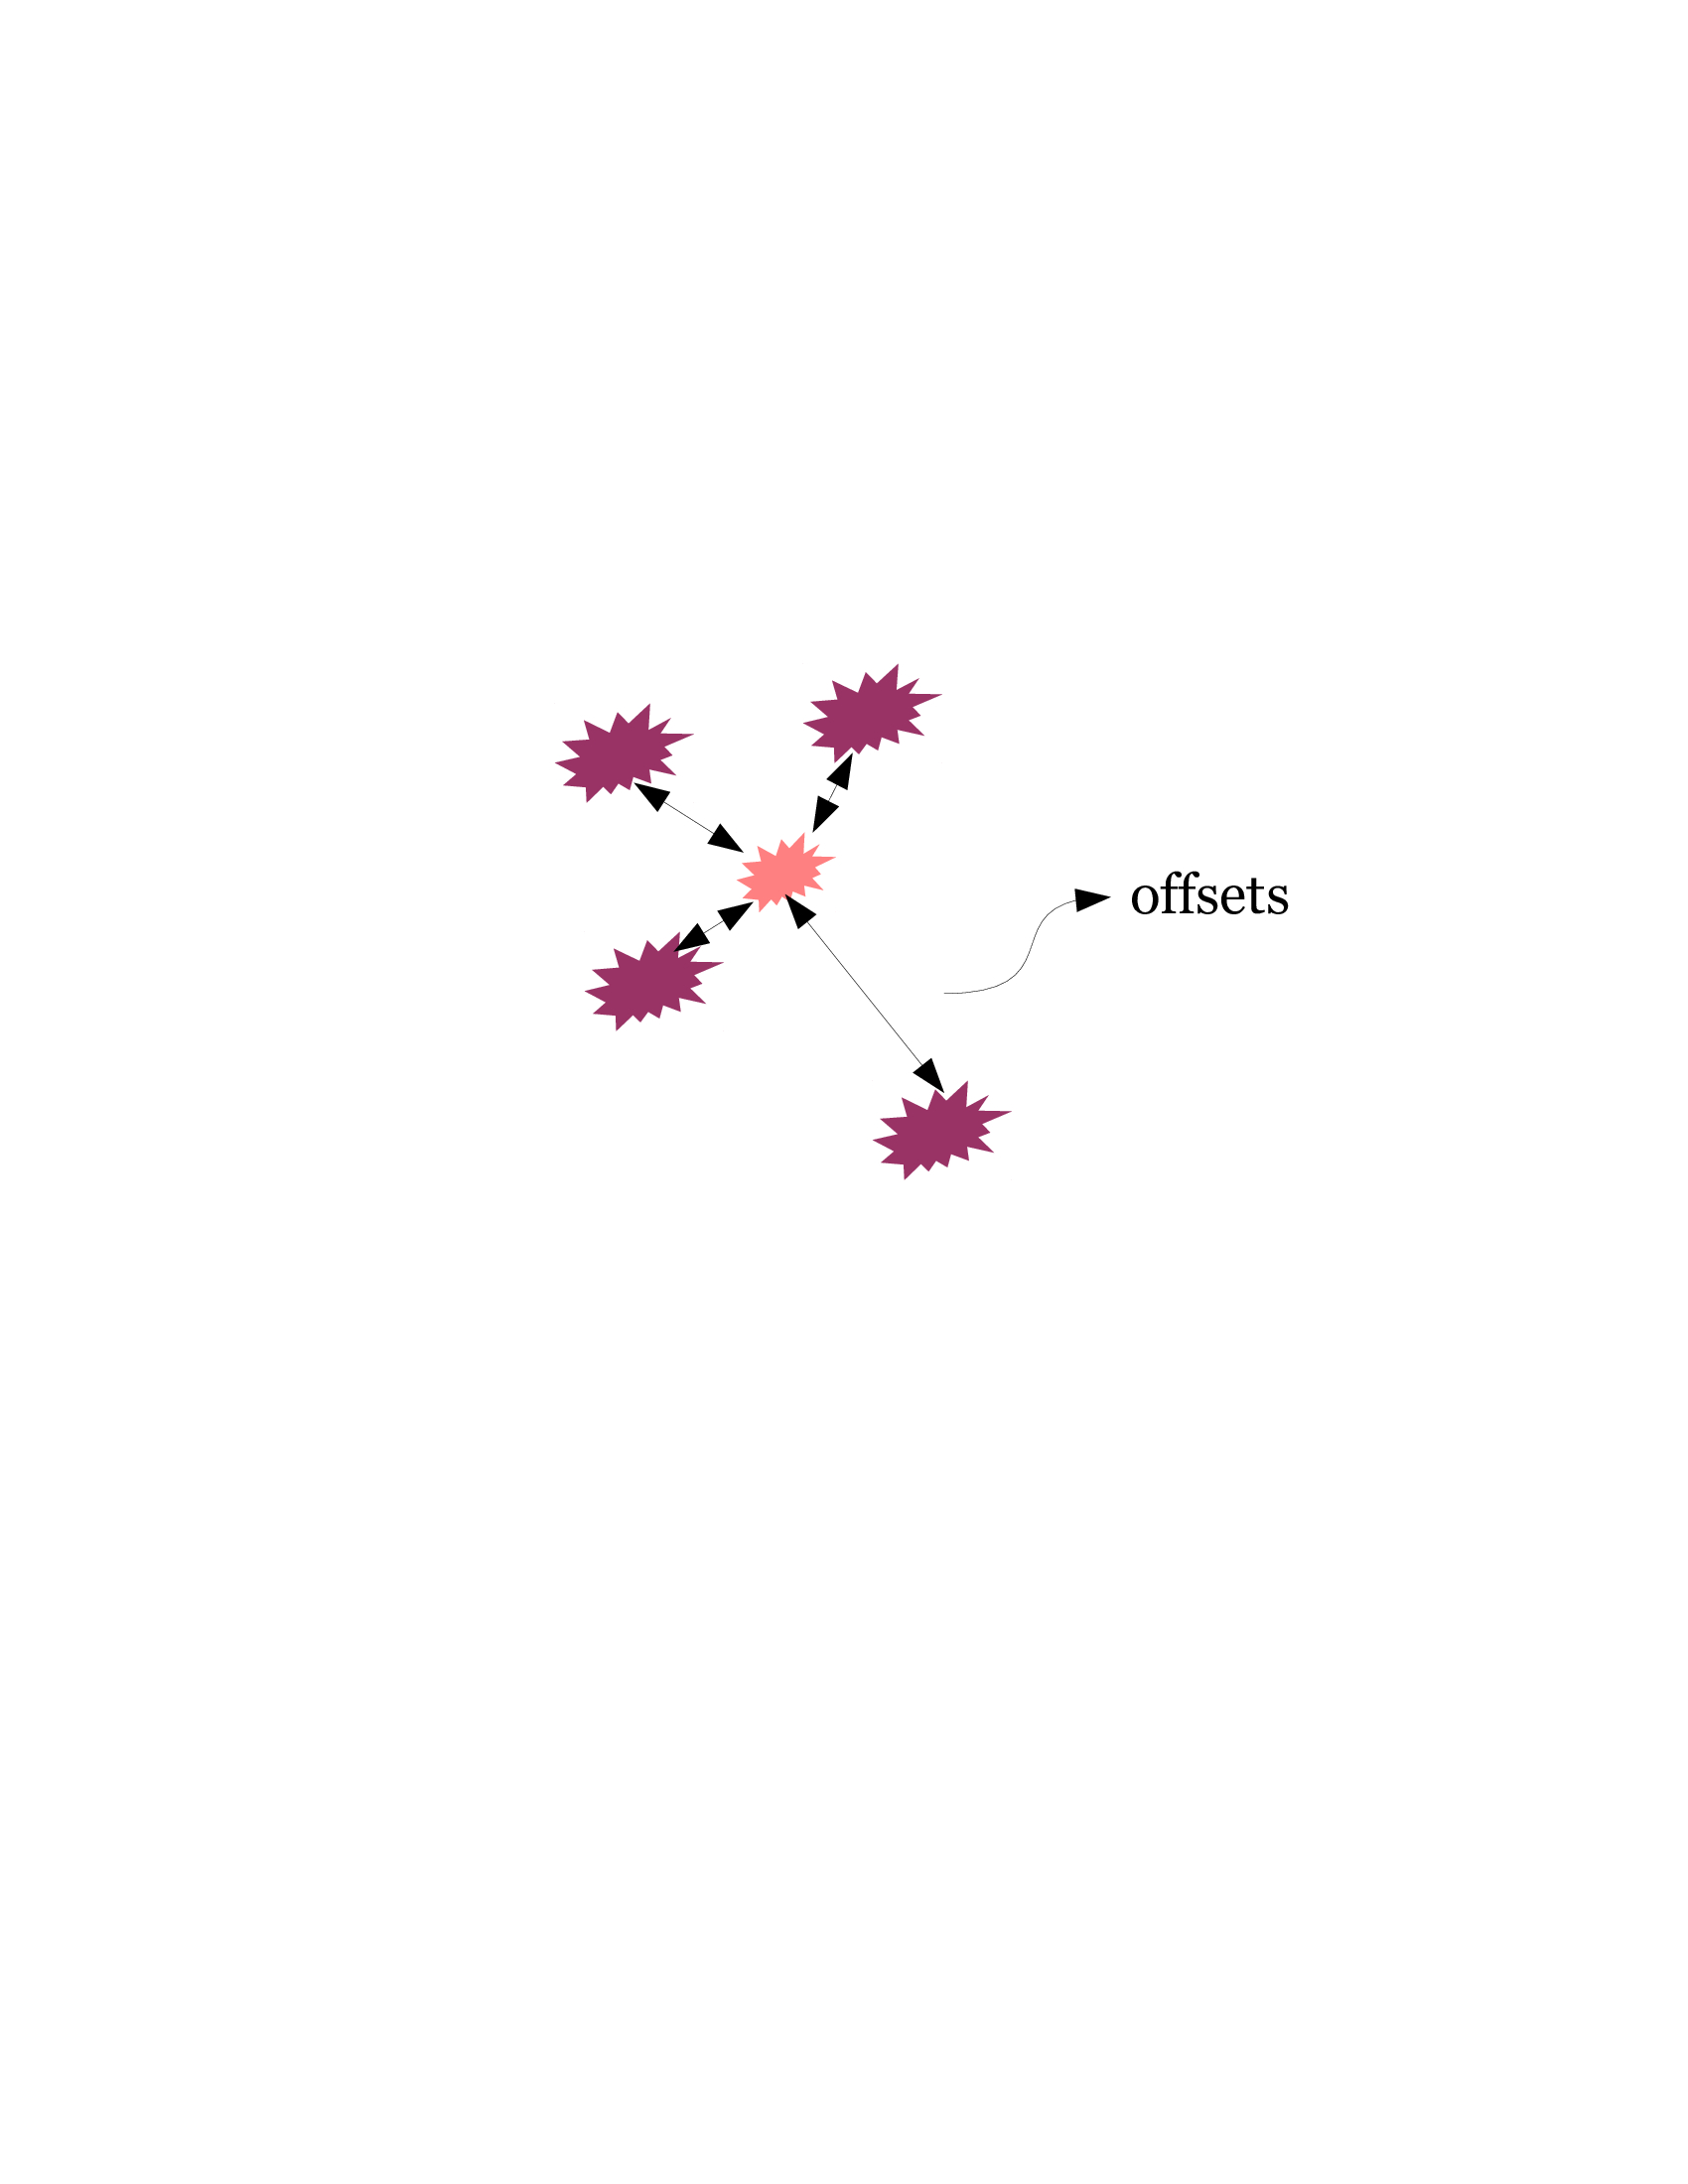
\includegraphics[width=0.5\textwidth]{3.jpg}\end{figure}
             \end{itemize}   
	\end{enumerate}
\end{frame}   


%\item<4-> We obtain a median position for each and find offsets. 
%                 \item<5-> We pixelize the data and for each pixel we average over galaxies within a radius of three times the size of the pixel. This translates to averaging over a $100$ galaxies in a $10$ arcminute radius.
%                  \item<6-> We obtain the final positions of galaxies by updating the previous positions by these averaged offsets.


\begin{frame}
\frametitle{Method Proposed}
	\begin{enumerate}
		\item Begin with the PanStarrs dataset
        \item Obtain a fixed background of galaxies : The Reference System
        	\begin{itemize}
				\item The data does seem to suggest that the galaxies 'move'
                \item four epochs, find a median value, find offsets, average using hundred galaxies.
               \end{itemize}
%         \item Finally obtain the differences in positions of stars
% 			\begin{itemize}
%                     \item  For every pixel of the sky, obtain offsets epoch-wise again averaged over galaxies within $10$ arcminutes.
%                     \item Find how much the stars have moved! 
% 			\end{itemize}
        
	\end{enumerate}
\end{frame}

% \begin{frame}
% \frametitle{haha}
% \begin{figure}
% \includegraphics[width=0.5\textwidth]{Untitled_1.jpg}
% \end{figure}

% \end{frame}

% \begin{frame}
% \frametitle{haha}
% \begin{figure}
% \includegraphics[width=0.5\textwidth]{Untitled_2.jpg}
% \end{figure}

% \end{frame}


% \begin{frame}
% \frametitle{haha}
% \begin{figure}
% \includegraphics[width=0.5\textwidth]{Untitled_3.jpg}
% \end{figure}

% \end{frame}

\begin{frame}
\frametitle{Detail}
\begin{figure}
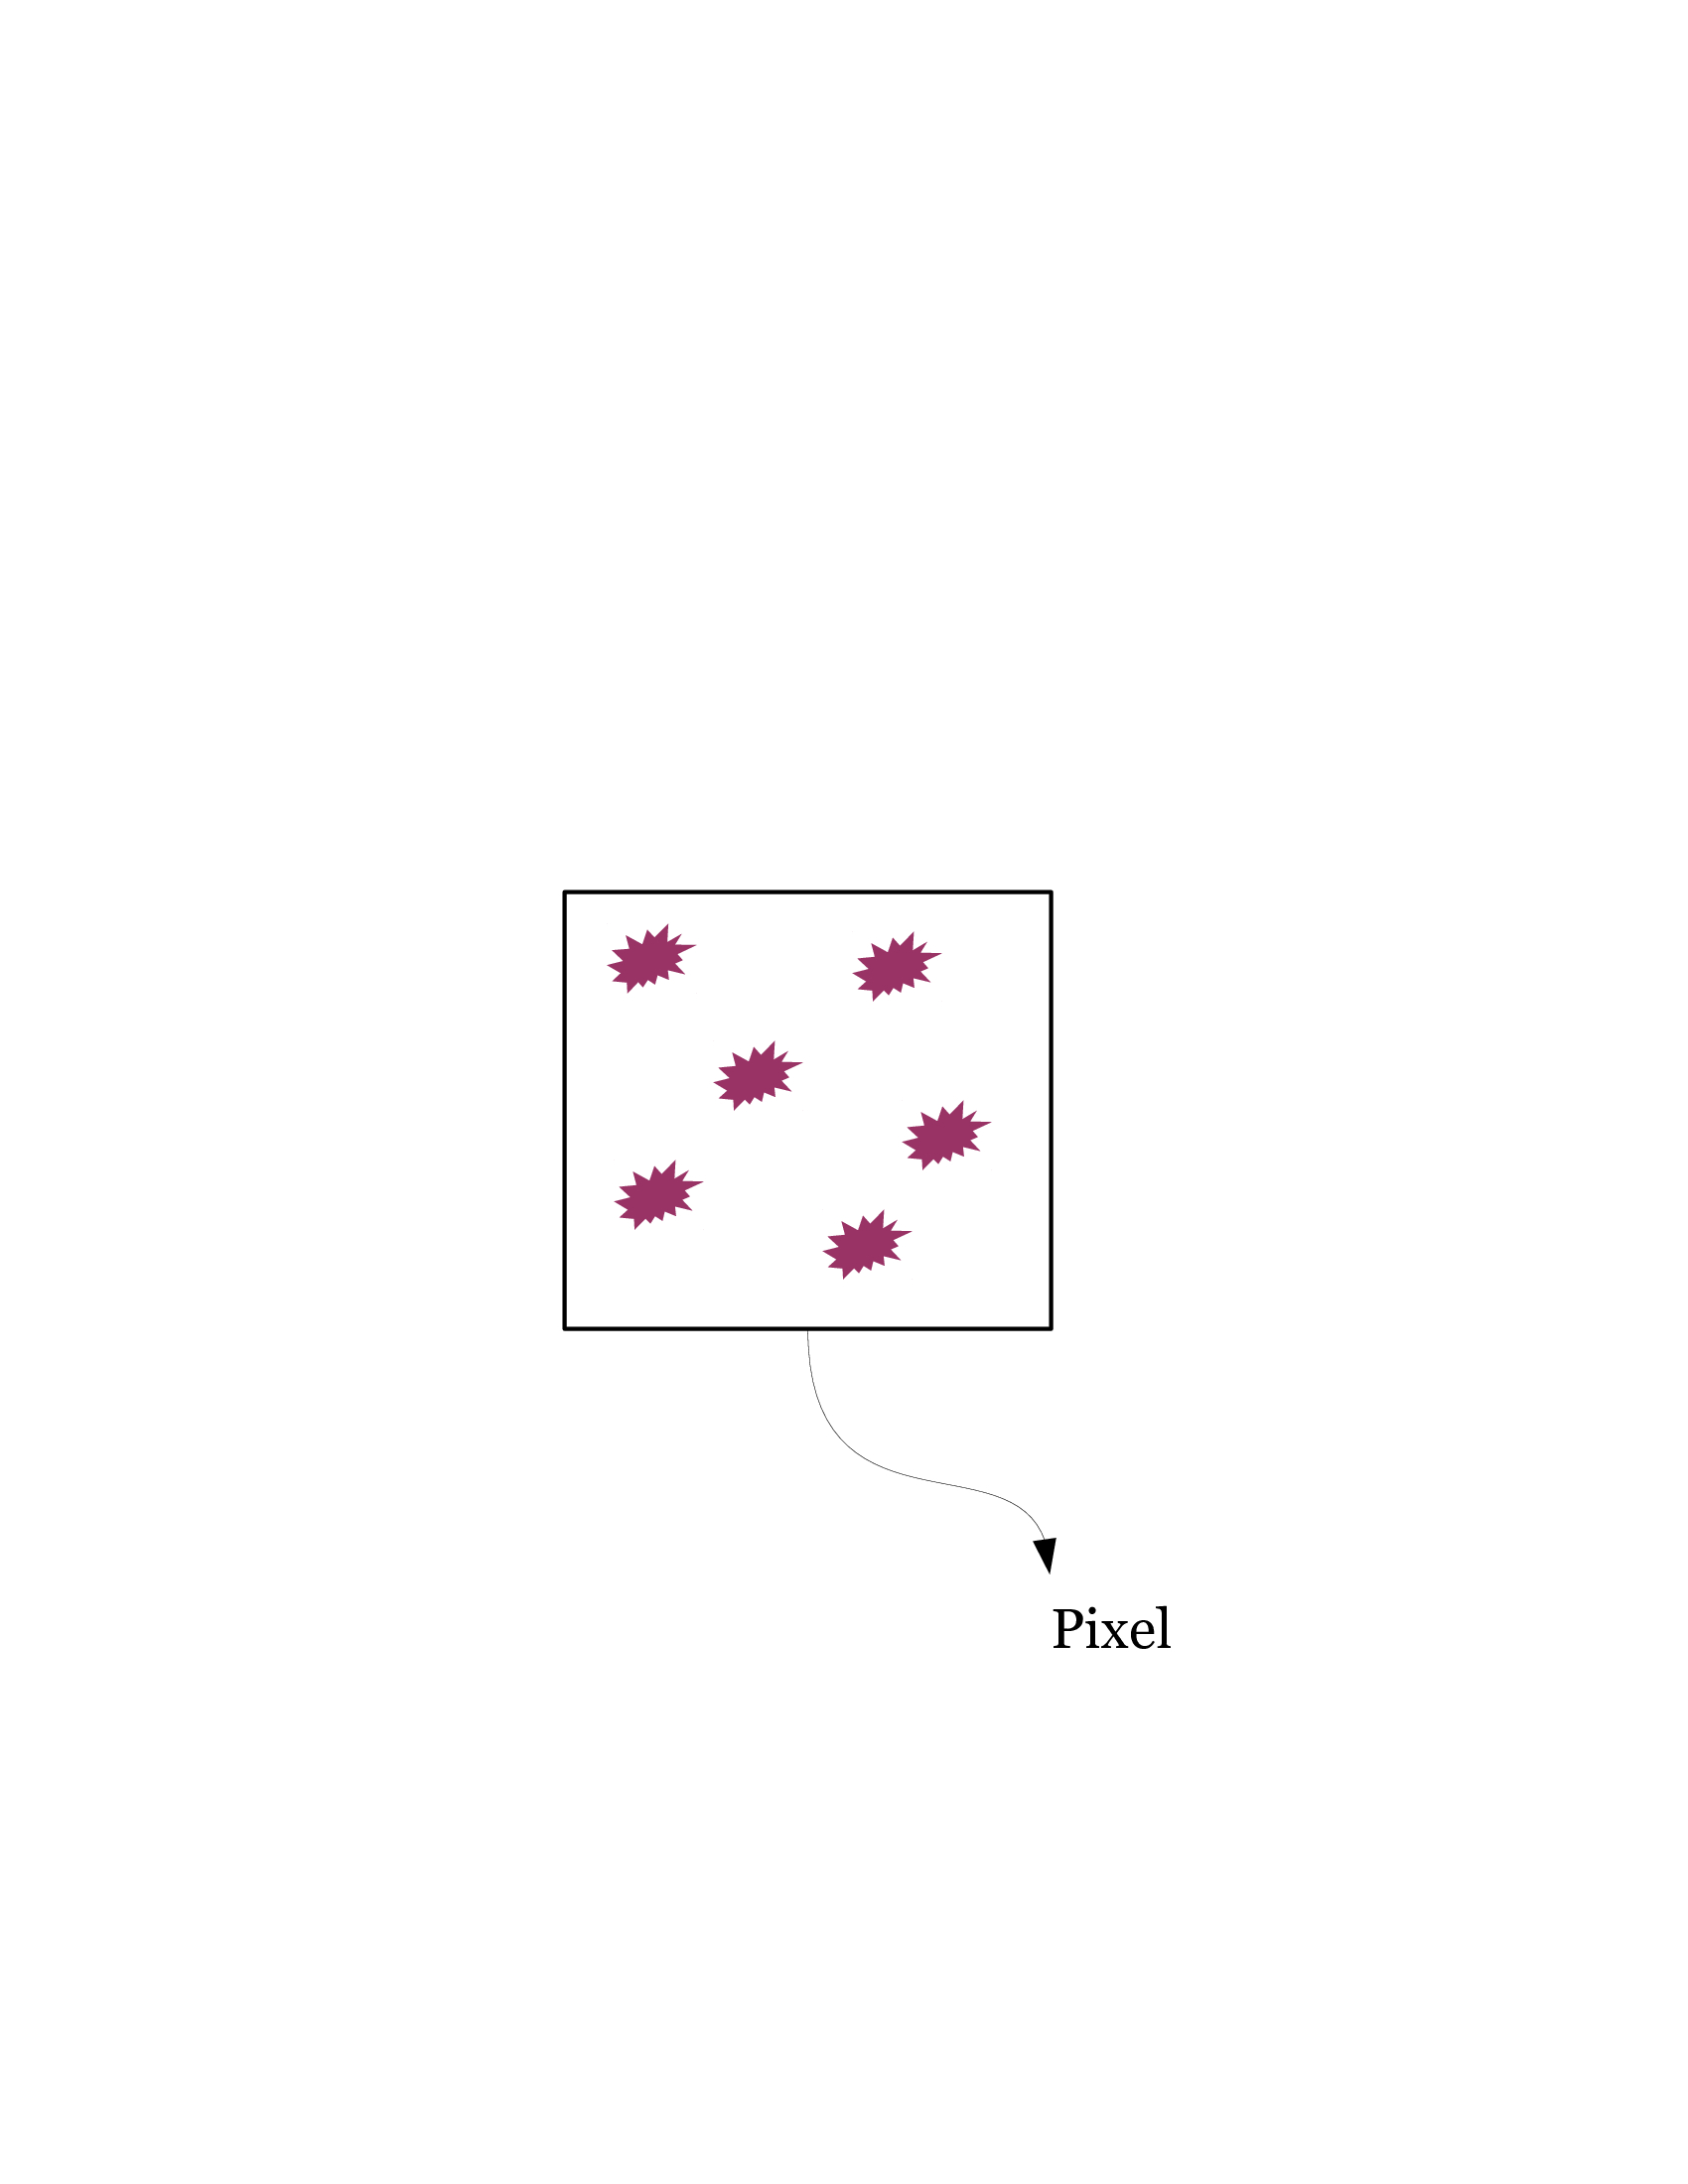
\includegraphics[width=0.5\textwidth]{pixel.jpg}
\end{figure}

\end{frame}

\begin{frame}
\frametitle{Detail}
\begin{figure}\centering
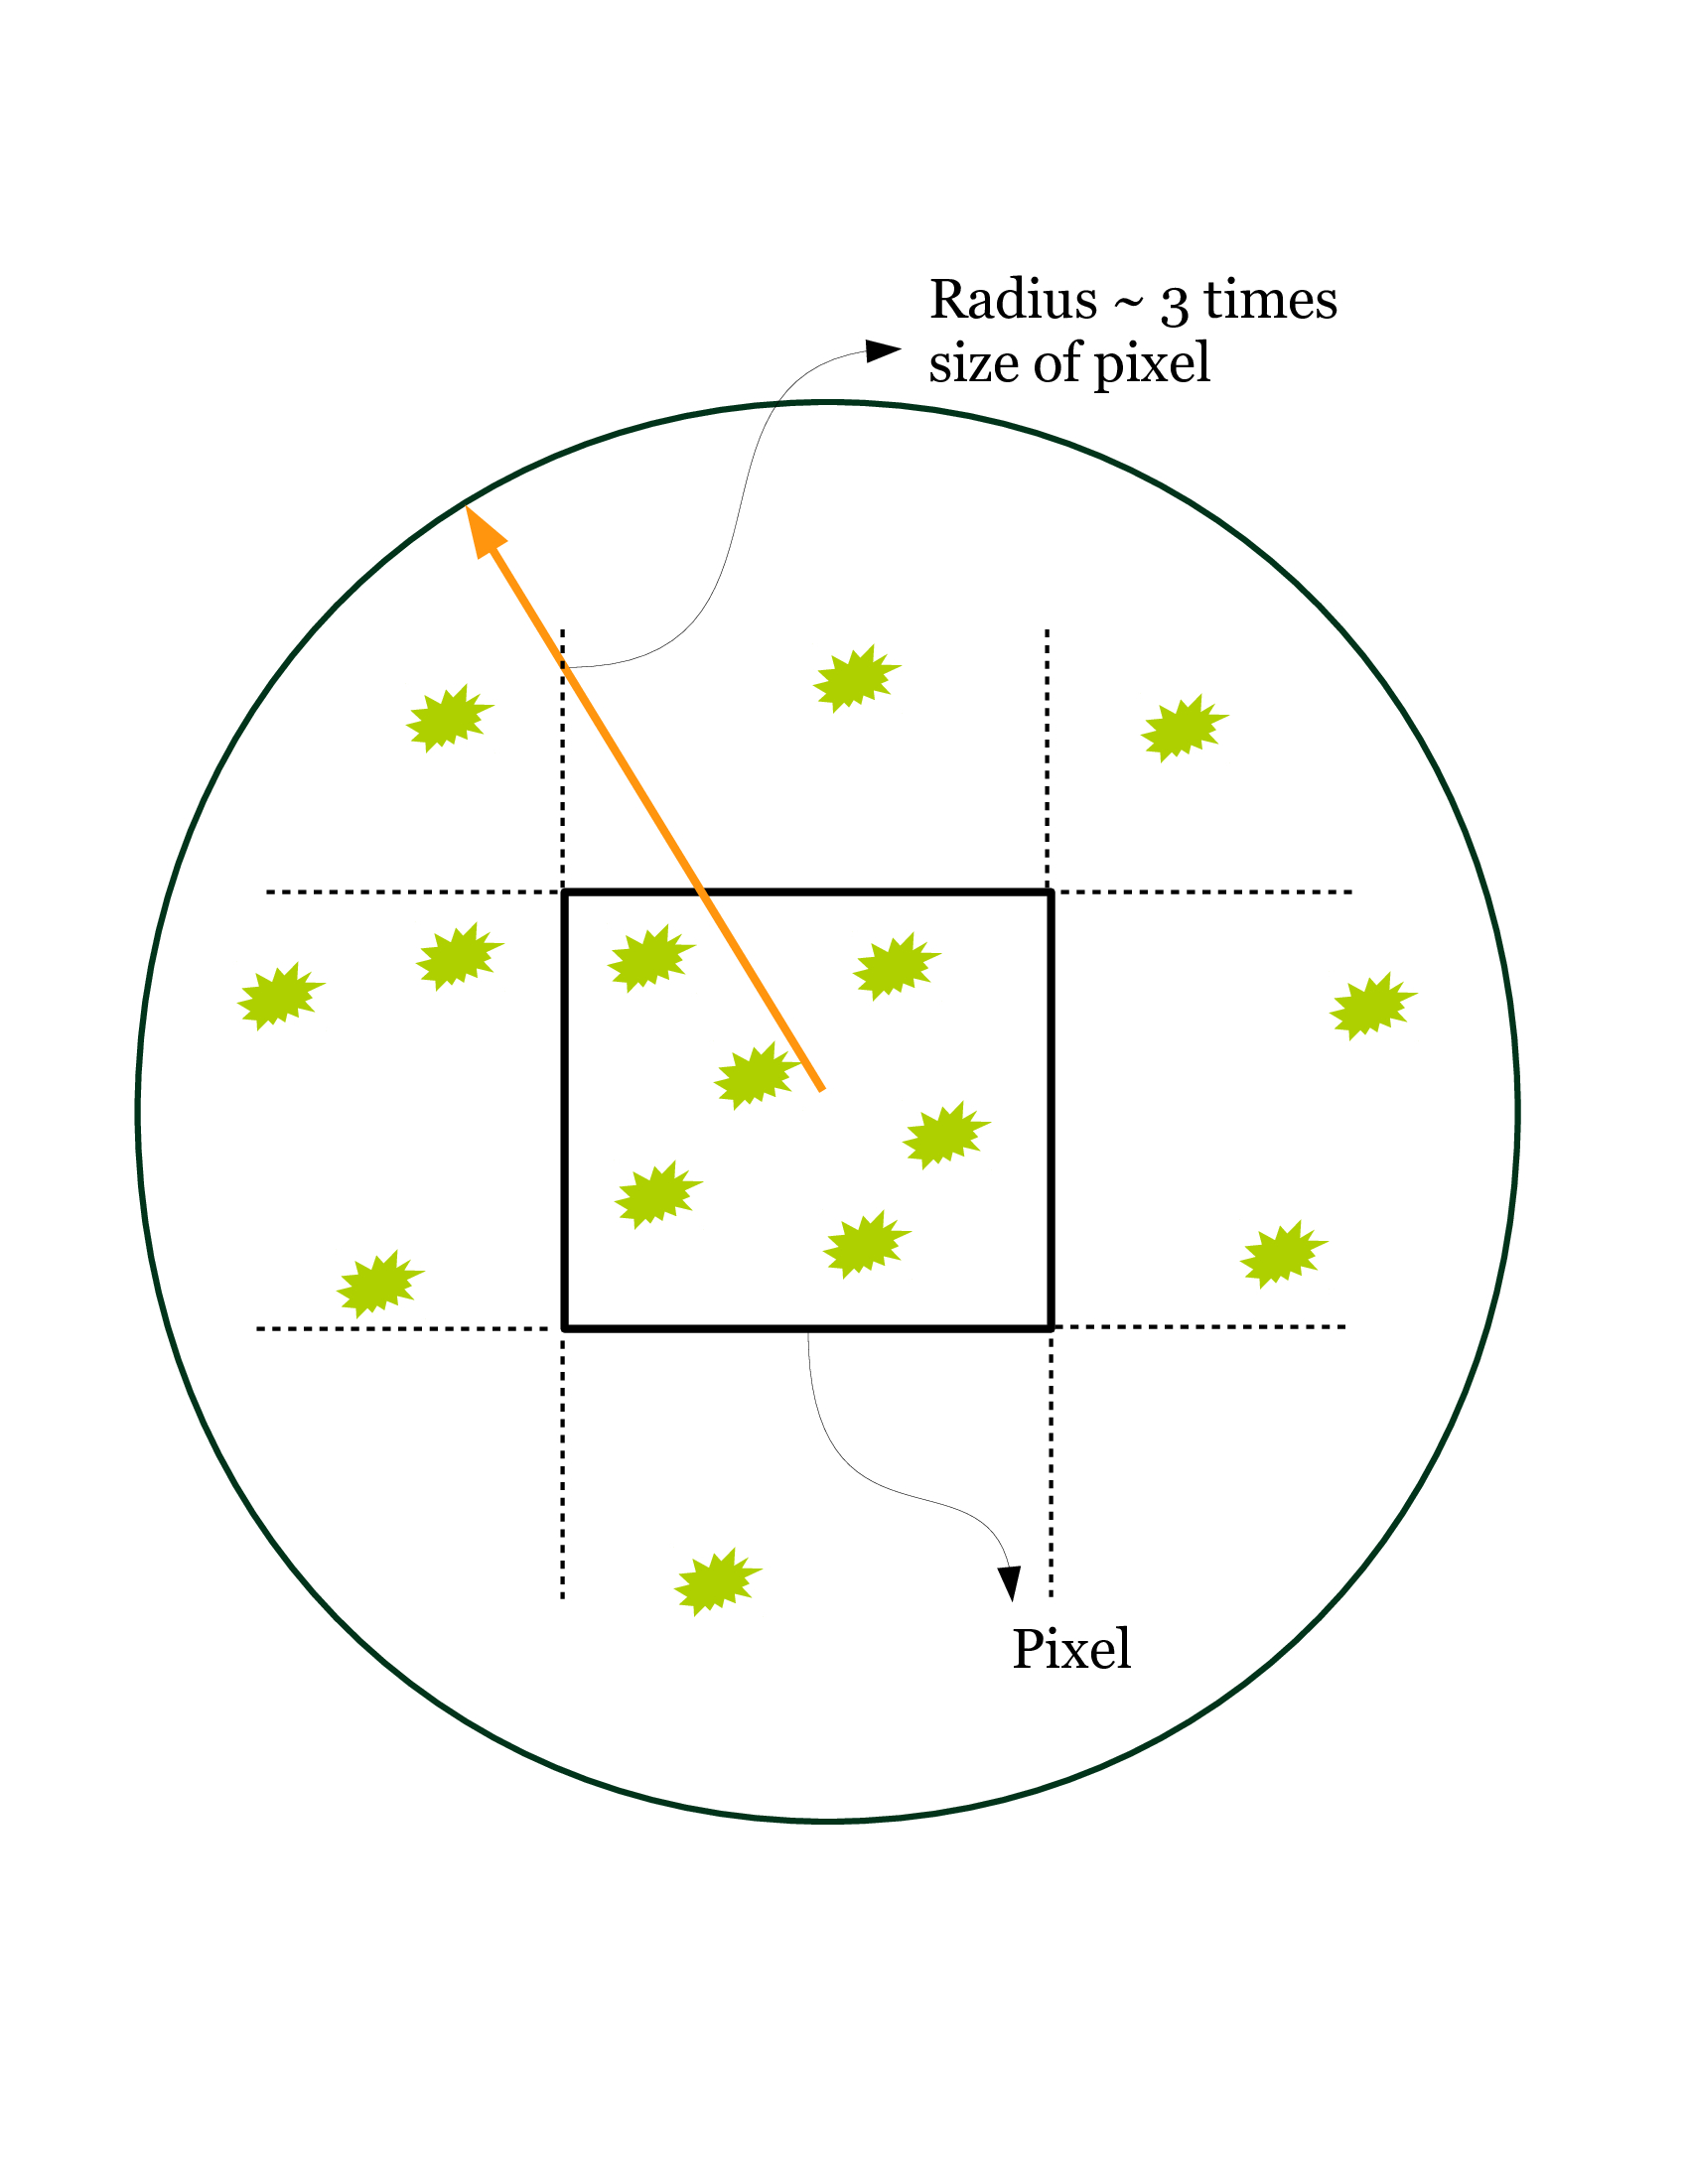
\includegraphics[width=0.5\textwidth, scale = 2.0]{pixelAndRadius.jpg}
\end{figure}

\end{frame}



\begin{frame}
\frametitle{Method Proposed}
	\begin{enumerate}
		\item Begin with the PanStarrs dataset
        \item Obtain a fixed background of galaxies : The Reference System
        	\begin{itemize}
				\item The data does seem to suggest that the galaxies 'move'
                \item four epochs, find a median value, find offsets, average using hundred galaxies.
                \item for each pixel, update the original position by the offset epochwise average.
               \end{itemize}
%         \item Finally obtain the differences in positions of stars
% 			\begin{itemize}
%                     \item  For every pixel of the sky, obtain offsets epoch-wise again averaged over galaxies within $10$ arcminutes.
%                     \item Find how much the stars have moved! 
% 			\end{itemize}
        
	\end{enumerate}
\end{frame}

\begin{frame}
\frametitle{Detail}
\begin{figure}\centering
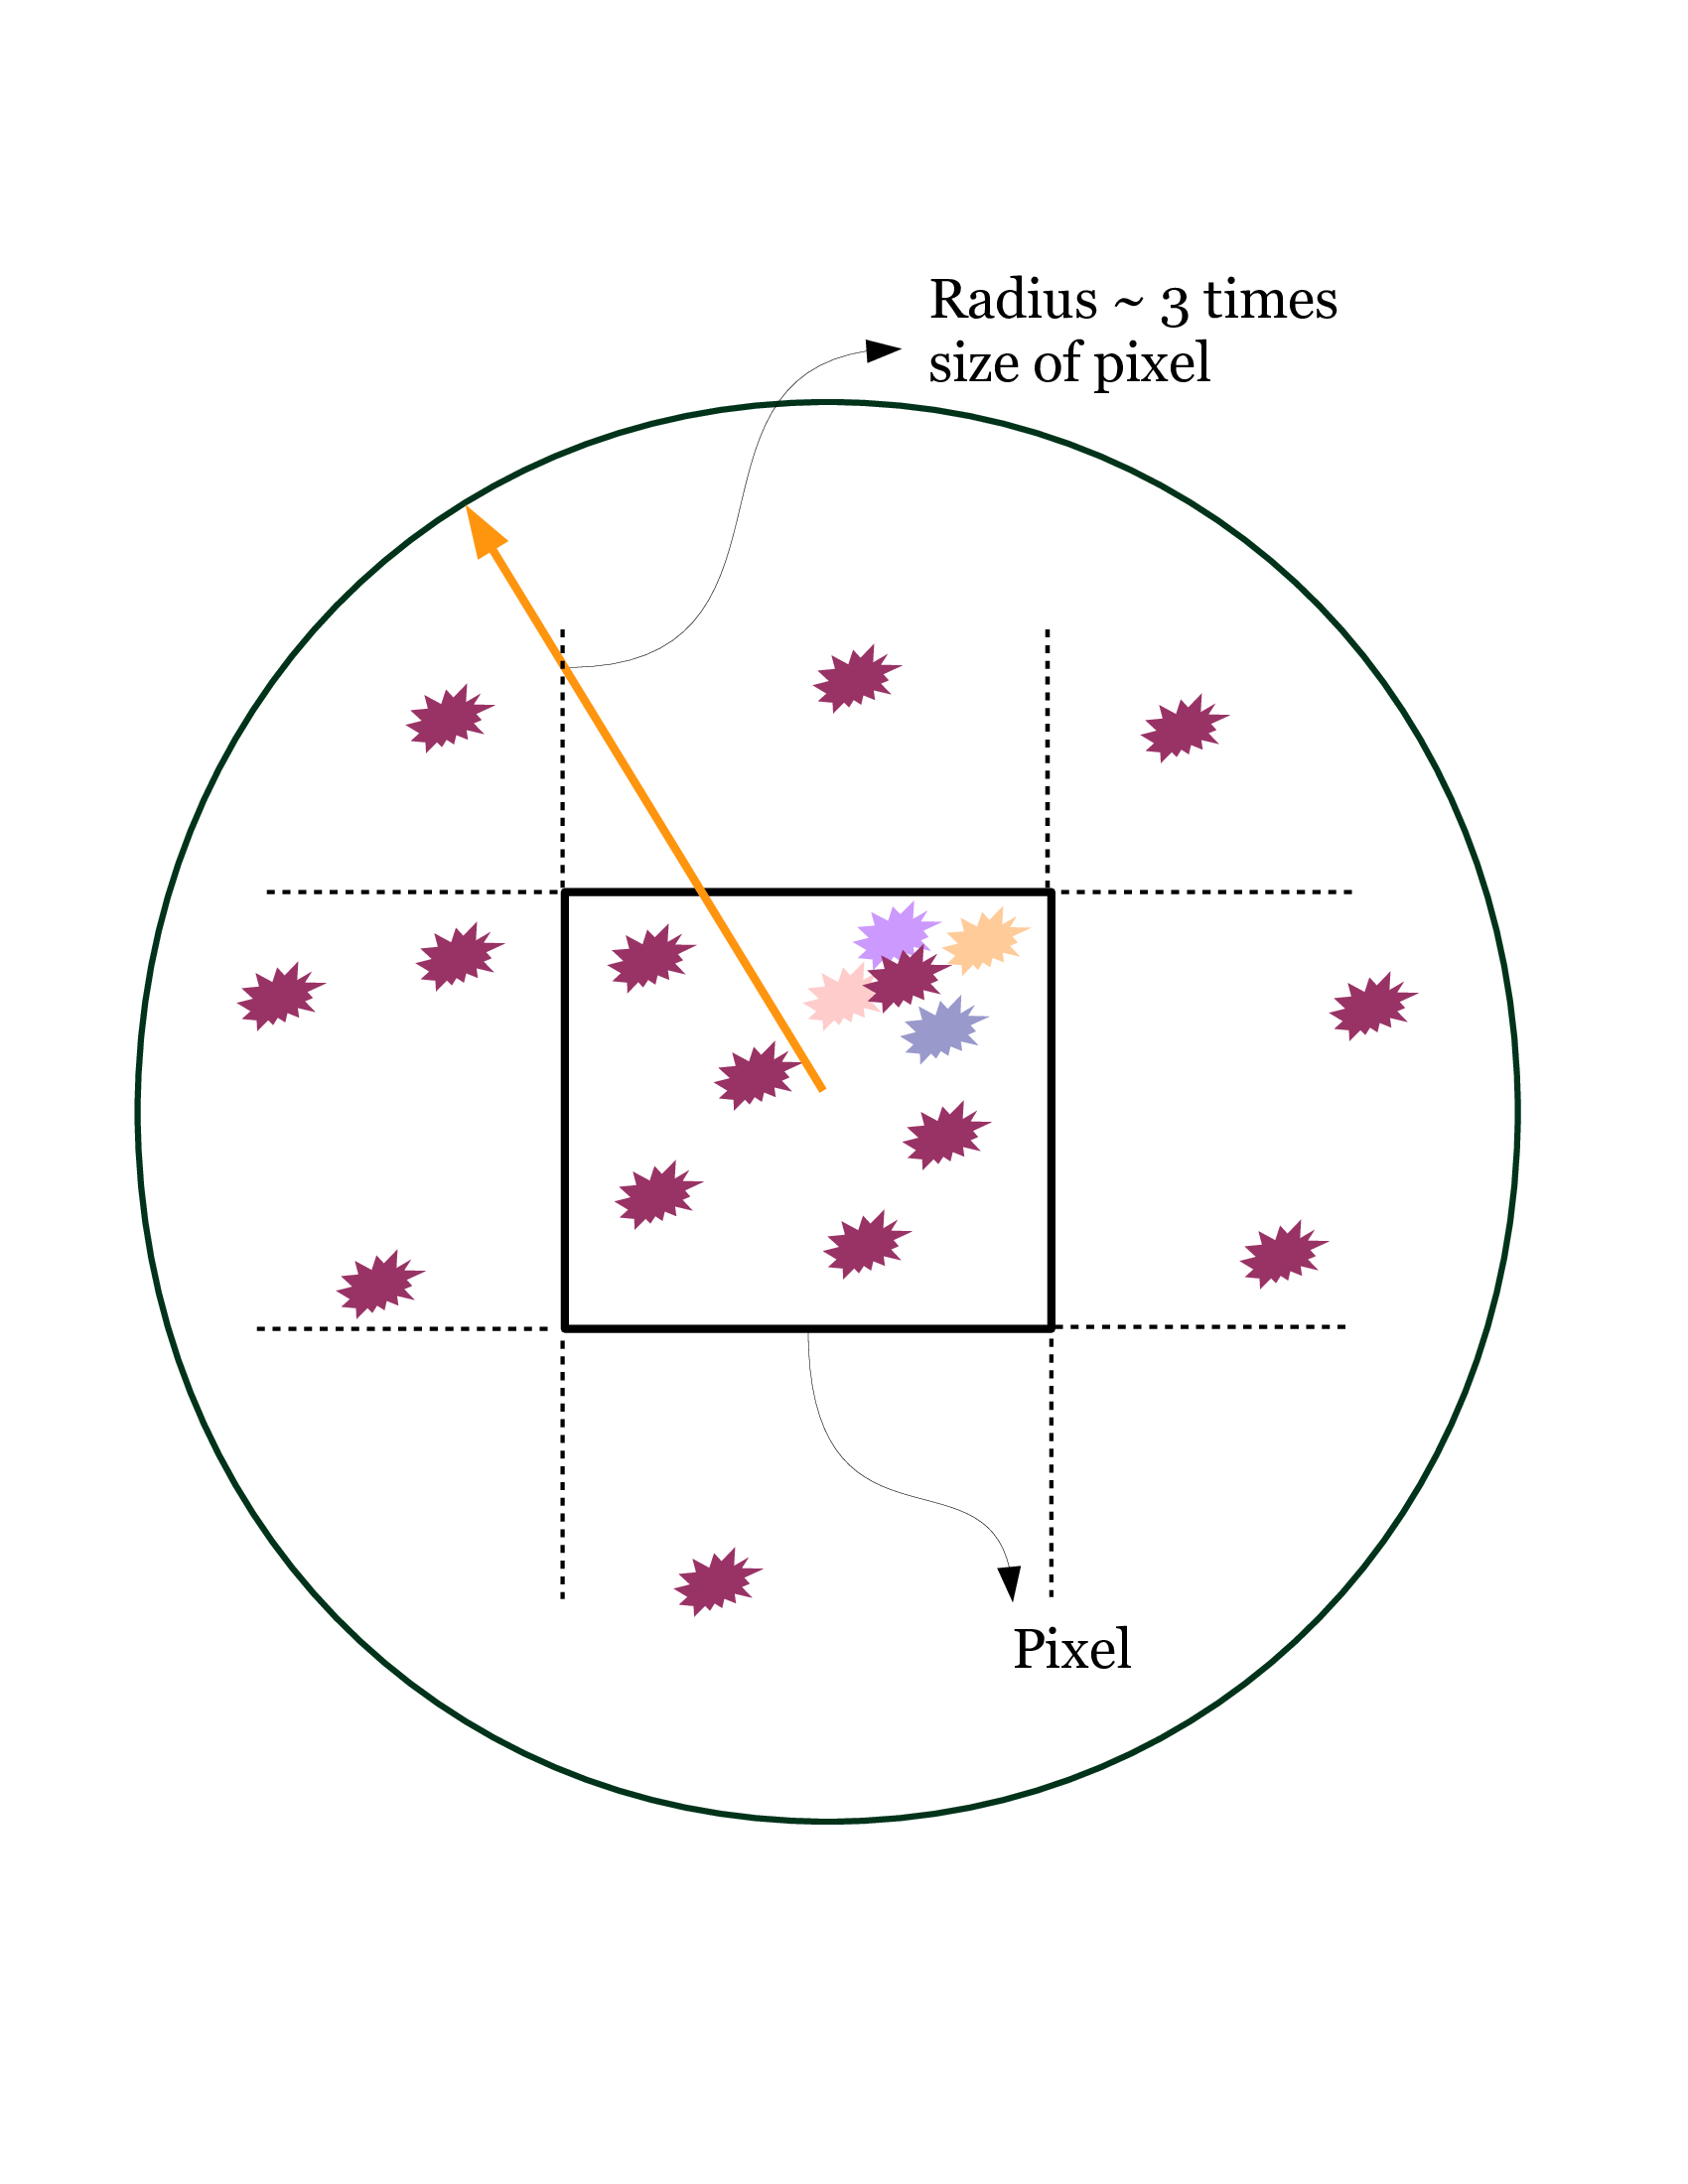
\includegraphics[width=0.5\textwidth]{pixelRadiusMedianAndOthers.jpg}
\end{figure}

\end{frame}



\begin{frame}
\frametitle{Method Proposed}
	\begin{enumerate}
		\item Begin with the PanStarrs dataset
        \item Obtain a fixed background of galaxies : The Reference System
        	\begin{itemize}
				\item The data does seem to suggest that the galaxies 'move'
                \item four epochs, find a median value, find offsets, average using hundred galaxies.
                \item for each pixel, update the original position by the offset epochwise average.
               \end{itemize}
        \item Finally calibrate positions of stars
% 			\begin{itemize}
%                     \item  For every pixel of the sky, obtain offsets epoch-wise again averaged over galaxies within $10$ arcminutes.
%                     \item Find how much the stars have moved! 
% 			\end{itemize}
        
	\end{enumerate}
\end{frame}


\begin{frame}
\frametitle{Detail}
\begin{figure}\centering
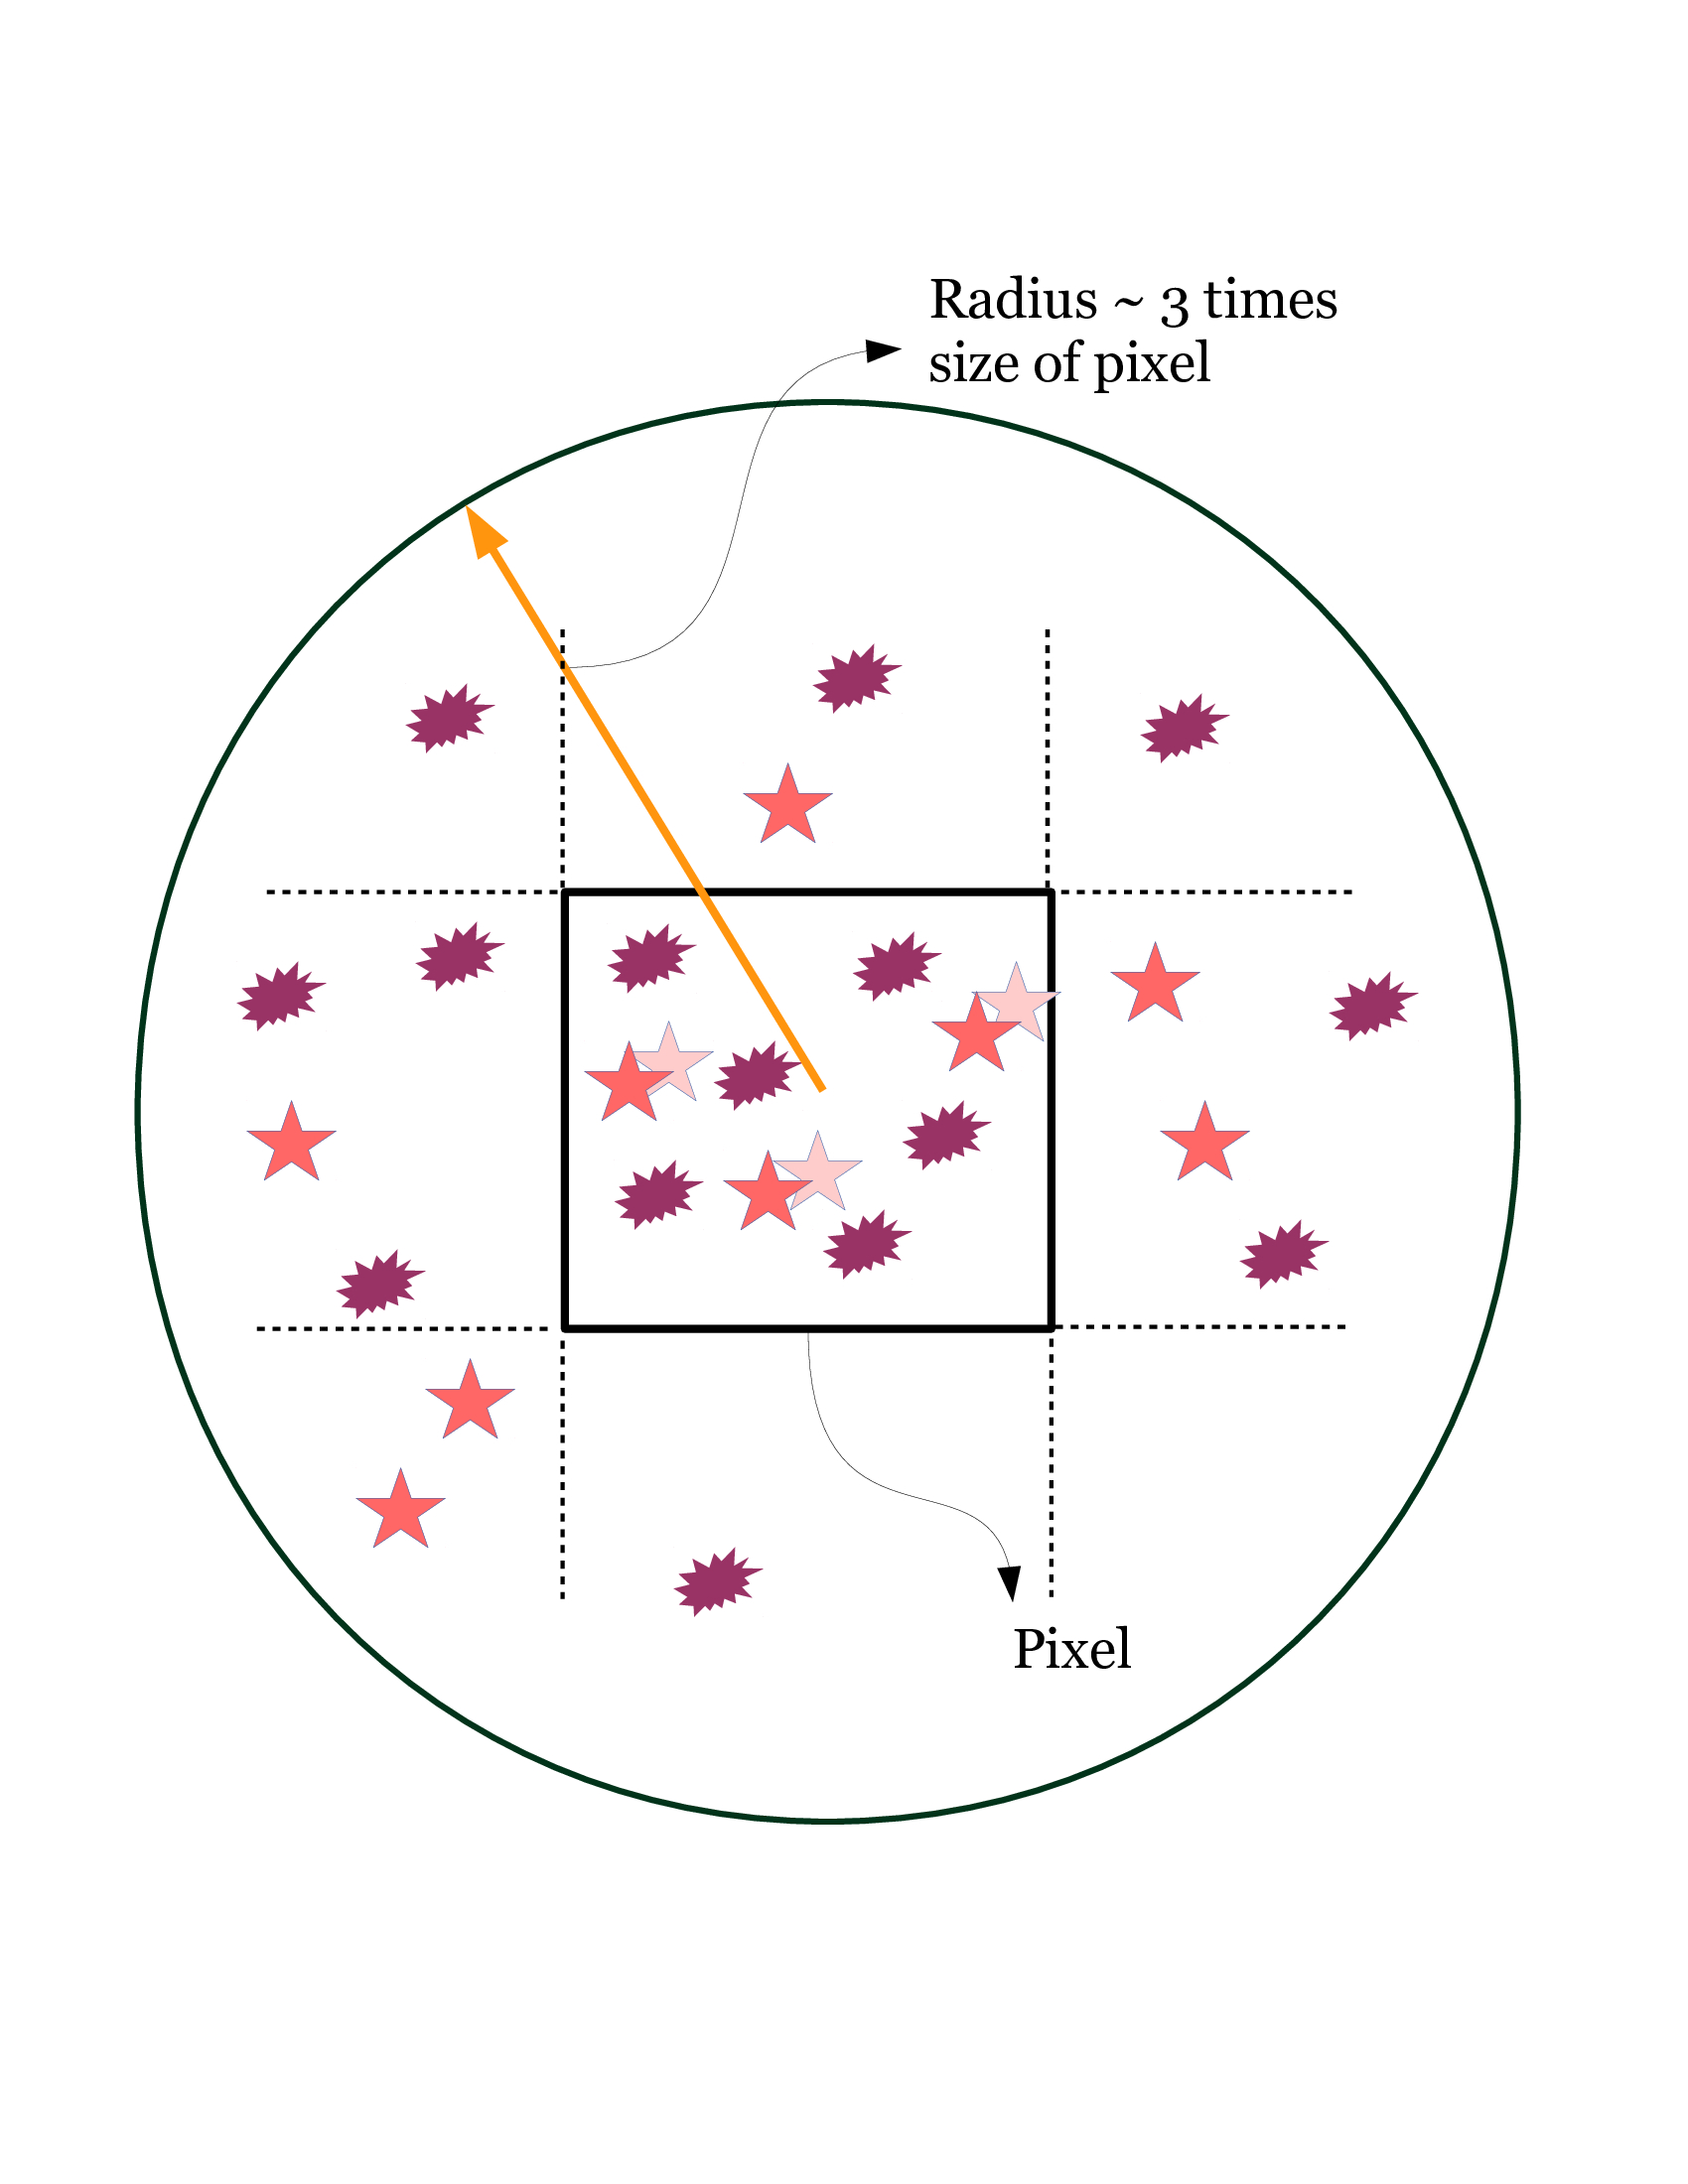
\includegraphics[width=0.5\textwidth]{pixelRadiusStarGalaxy.jpg}
\end{figure}

\end{frame}

\begin{frame}
\frametitle{edge effects}
\begin{figure}\centering
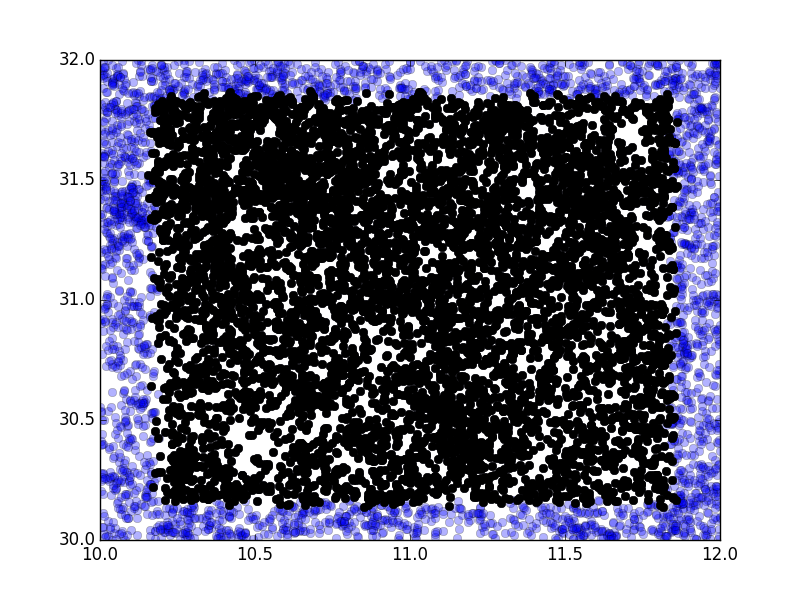
\includegraphics[width=0.5\textwidth]{edgeEffects.png}
\end{figure}

\end{frame}

%%%%%%%%%%%%%%%%%%%%%%%%%%%%%%%%%%%%%%
\section{Progress}

\begin{frame}
\frametitle{achieved goals}
	\begin{itemize}
		\item<1-> We begin with the PanStarrs dataset. The other datasets are largely similar and would follow easily. 
        \item<2-> We download data using lsd and store it in h5 files. The downloading of data is done as and when the chunks of sky are loaded.  
        \item<3->The code for fixing galaxies as the background has been written. 
        \item<4-> The code for calculating movement of stars given the fixed background has been written. 
        \item<5-> The final data will be stored in database format. 
	\end{itemize}
\end{frame}

\begin{frame}
\frametitle{bugs}
	\begin{itemize}
		\item<1-> $numpy.in1d(ar1, ar2, assume\_unique=False, invert=False)$
         Test whether each element of a 1-D array is also present in a second array.
    Returns a boolean array the same length as `ar1` that is True
    where an element of `ar1` is in `ar2` and False otherwise. \\
      
	
	\item<2-> fixed it using the python library 'pandas' \textit{IndexError: unsupported iterator index}  -- maybe not compatible with numpy :(
	\end{itemize}
\end{frame}


\begin{frame}
\frametitle{future goals}
	\begin{itemize}
		\item<1-> Complete debugging of code and obtain the database for PanStarrs.
        \item<2-> Move on to the other datasets and finally obtain proper motions of stars under consideration.
	\end{itemize}
\end{frame}





% \begin{frame}[fragile]
%   \frametitle{mtheme}

%   The \emph{mtheme} is a Beamer theme with minimal visual noise inspired by the
%   \href{https://github.com/hsrmbeamertheme/hsrmbeamertheme}{\textsc{hsrm} Beamer
%   Theme} by Benjamin Weiss.

%   Enable the theme by loading

%   \begin{minted}[fontsize=\small]{latex}
%     \documentclass{beamer}
%     \usetheme{m}
%   \end{minted}

%   Note, that you have to have Mozilla's \emph{Fira Sans} font and XeTeX
%   installed to enjoy this wonderful typography.
% \end{frame}

% \begin{frame}[fragile]
%   \frametitle{Sections}
%   Sections group slides of the same topic

%   \begin{minted}[fontsize=\small]{latex}
%     \section{Elements}
%   \end{minted}

%   for which the \emph{mtheme} provides a nice progress indicator \ldots
% \end{frame}

% \section{Elements}

% \begin{frame}[fragile]
%   \frametitle{Typography}
%       \begin{minted}[fontsize=\small]{latex}
% The theme provides sensible defaults to \emph{emphasize}
% text, \alert{accent} parts or show \textbf{bold} results.
%       \end{minted}

%   \begin{center}becomes\end{center}

%   The theme provides sensible defaults to \emph{emphasize} text,
%   \alert{accent} parts or show \textbf{bold} results.
% \end{frame}
% \begin{frame}{Lists}
%   \begin{columns}[onlytextwidth]
%     \column{0.5\textwidth}
%       Items
%       \begin{itemize}
%         \item Milk \item Eggs \item Potatos
%       \end{itemize}

%     \column{0.5\textwidth}
%       Enumerations
%       \begin{enumerate}
%         \item First, \item Second and \item Last.
%       \end{enumerate}
%   \end{columns}
% \end{frame}
% \begin{frame}{Descriptions}
%   \begin{description}
%     \item[PowerPoint] Meeh.
%     \item[Beamer] Yeeeha.
%   \end{description}
% \end{frame}
% \begin{frame}{Animation}
%   \begin{itemize}[<+- | alert@+>]
%     \item \alert<4>{This is\only<4>{ really} important}
%     \item Now this
%     \item And now this
%   \end{itemize}
% \end{frame}
% \begin{frame}{Figures}
%   \begin{figure}
%     \newcounter{density}
%     \setcounter{density}{20}
%     \begin{tikzpicture}
%       \def\couleur{mLightBrown}
%       \path[coordinate] (0,0)  coordinate(A)
%                   ++( 90:5cm) coordinate(B)
%                   ++(0:5cm) coordinate(C)
%                   ++(-90:5cm) coordinate(D);
%       \draw[fill=\couleur!\thedensity] (A) -- (B) -- (C) --(D) -- cycle;
%       \foreach \x in {1,...,40}{%
%           \pgfmathsetcounter{density}{\thedensity+20}
%           \setcounter{density}{\thedensity}
%           \path[coordinate] coordinate(X) at (A){};
%           \path[coordinate] (A) -- (B) coordinate[pos=.10](A)
%                               -- (C) coordinate[pos=.10](B)
%                               -- (D) coordinate[pos=.10](C)
%                               -- (X) coordinate[pos=.10](D);
%           \draw[fill=\couleur!\thedensity] (A)--(B)--(C)-- (D) -- cycle;
%       }
%     \end{tikzpicture}
%     \caption{Rotated square from
%     \href{http://www.texample.net/tikz/examples/rotated-polygons/}{texample.net}.}
%   \end{figure}
% \end{frame}
% \begin{frame}{Tables}
%   \begin{table}
%     \caption{Largest cities in the world (source: Wikipedia)}
%     \begin{tabular}{lr}
%       \toprule
%       City & Population\\
%       \midrule
%       Mexico City & 20,116,842\\
%       Shanghai & 19,210,000\\
%       Peking & 15,796,450\\
%       Istanbul & 14,160,467\\
%       \bottomrule
%     \end{tabular}
%   \end{table}
% \end{frame}
% \begin{frame}{Blocks}

%   \begin{block}{This is a block title}
%     This is soothing.
%   \end{block}

% \end{frame}
% \begin{frame}{Math}
%   \begin{equation*}
%     e = \lim_{n\to \infty} \left(1 + \frac{1}{n}\right)^n
%   \end{equation*}
% \end{frame}
% \begin{frame}{Line plots}
%   \begin{figure}
%     \begin{tikzpicture}
%       \begin{axis}[
%         mlineplot,
%         width=0.9\textwidth,
%         height=6cm,
%       ]

%         \addplot {sin(deg(x))};
%         \addplot+[samples=100] {sin(deg(2*x))};

%       \end{axis}
%     \end{tikzpicture}
%   \end{figure}
% \end{frame}
% \begin{frame}{Bar charts}
%   \begin{figure}
%     \begin{tikzpicture}
%       \begin{axis}[
%         mbarplot,
%         xlabel={Foo},
%         ylabel={Bar},
%         width=0.9\textwidth,
%         height=6cm,
%       ]

%       \addplot plot coordinates {(1, 20) (2, 25) (3, 22.4) (4, 12.4)};
%       \addplot plot coordinates {(1, 18) (2, 24) (3, 23.5) (4, 13.2)};
%       \addplot plot coordinates {(1, 10) (2, 19) (3, 25) (4, 15.2)};

%       \legend{lorem, ipsum, dolor}

%       \end{axis}
%     \end{tikzpicture}
%   \end{figure}
% \end{frame}
% \begin{frame}{Quotes}
%   \begin{quote}
%     Veni, Vidi, Vici
%   \end{quote}
% \end{frame}


\section{Colophon}

\begin{frame}{colophon}

	This work is available at 
    
    \begin{center}\url{github.com/prashansa/properMotions}\end{center} 

%   Get the source of this theme and the demo presentation from

%   \begin{center}\url{github.com/matze/mtheme}\end{center}

  The theme \emph{itself} is licensed under a
  \href{http://creativecommons.org/licenses/by-sa/4.0/}{Creative Commons
  Attribution-ShareAlike 4.0 International License}.

  \begin{center}\ccbysa\end{center}

\end{frame}

\plain{Questions?}

\end{document}